\documentclass{report}

\usepackage[english]{babel}
\usepackage[latin1]{inputenc}
\usepackage[T1]{fontenc}
\usepackage {graphicx}
\usepackage{subcaption}
\usepackage{threeparttable}
\usepackage{placeins}
\usepackage{amsmath}
\usepackage[makeroom]{cancel}
\usepackage{tikz}
\usetikzlibrary{arrows,automata}
\usepackage{multirow}

%

\author{
  Sim�es, Jo�o\\
  197311\\
  \texttt{joao.simoes@tu-dortmund.de}
  \and
  Louren�o, Bernardo\\
  197214\\
  \texttt{bernardo.lourenco@tu-dortmund.de}
  \and
  Kamenca, Tomas\\
  199715\\
  \texttt{tomas.kamenca@tu-dortmund.de}
  \and
  Alias, Nil\\
  197167\\
  \texttt{nil.alias@tu-dortmund.de}
}
\title{\Huge MaschinenbauInformatik \\\Huge Mini-Robot}
\date{Date of Submission: \today}

\begin{document}
%
 
%\maketitle
\begin{titlepage}
\centering
	\includegraphics[width=0.15\textwidth]{itpllogo}\par\vspace{1cm}
	{\scshape\LARGE TU Dortmund \par}
	%\vspace{1cm}
	{\scshape\Large Maschinenbauinformatik Project\par}
	\vspace{1.5cm}
	{\huge\bfseries Mini-Robot\par}
	\vspace{1cm}
	\Large{Project by:}\\
	\vspace{0.3cm}

	\centering
  Sim�es, Jo�o\hspace{1cm}197311\\
  \texttt{joao.simoes@tu-dortmund.de}\\
\vspace{0.2cm}
  Louren�o, Bernardo\hspace{1cm}197214\\
  \texttt{bernardo.lourenco@tu-dortmund.de}\\
\vspace{0.2cm} 
  Kamenca, Tomas\hspace{1cm}199715\\
  \texttt{tomas.kamenca@tu-dortmund.de}\\
\vspace{0.2cm}
  Alias, Nil\hspace{1cm}197167\\
  \texttt{nil.alias@tu-dortmund.de}

	\vfill
	Task assigned by\par
	Dipl.-Inf. Dominik Schmitt\\
	Univ.-Prof. Dr.-Ing. Markus Rabe

	\vfill

% Bottom of the page
	{\large \today\par}
\end{titlepage}


\tableofcontents

\listoffigures

\listoftables

\pagebreak
%

\chapter*{The Team}
The team consists of 4 Erasmus students from different backgrounds:
\paragraph{Jo�o Henrique Bernardo Sim�es}
Erasmus Student from University of Aveiro. Currently doing a Masters in Mechanical Engineering. Originally from Aveiro, Portugal and 21 years old. Little previous contact with micro-controllers, Basic C programming skills. 

\paragraph{Bernardo Miguel Martins Louren�o}
Erasmus student from University of Aveiro.  Currently doing Masters in Mechanical Engineering. Originally from Palha�a, Portugal and 23 years old. Intermidiate skills in C programming and frequent contact with micro-controllers (Arduino and PIC32)

\paragraph{Nil Al�as Botifoll}
Erasmus Student from Polytechnic University of Catalonia, Spain. Completed his bachelors degree in 2015 and currently finishing his masters degree in Industrial Engineering. Basic knowledge of C++ programming, sensors and micro-controllers, but willingness to learn.

\paragraph{Tomas Kamenca}
Erasmus Student from INSA Lyon, France. Currently doing a Master in Mechanical Engineering. Originally from Bratislava, Slovakia. Basic knowledge of C++, Java programming and micro-controllers.


\chapter{Introduction}

\section{Task}

\subsection{Given Task}
Our task is to design, build and control a robot.  The robot must be able to follow a given path without mechanical guidance from the outside. The robot must also be able to have some sort of interface in which the user can request a desired output. The use of 2 kinds of sensors, a display module and buttons is mandatory.
We were also given the option of making the robot able to overcome a list of more difficult challenges.

\subsection{Limitations}
Before clearly defining the objectives we have for this project we had to take into consideration our limitations. The budget, the lack of tools we have due to our Erasmus background, the lack of experience some members of our team have with this subject and the short time we have to complete this task due to our early departure were the main limitations that led us to keep our project simple, cost-effective and spend some extra time researching and designing the robot.

\subsection{Objectives}
\label{subsec:obj}
For the main task we decided that the path would be a black line taped to a white floor, the robot must be able to distinguish between the black path and the white background. In the task formulation in addition the the main task we were given the freedom of implementing many optional features to the robot. Because we have to use 2 kind of sensors we decided that we would should make the robot able to overcome something more than the base task. In addition to the main task, we decided we wanted the robot to be able to navigate around an unlooped maze and be able to find its output/Goal taped to the floor. Then go all the way back to the starting point and take an optimized path back to the end of the maze. The robot should be able to this while avoiding a possible obstacle and will be able to recognize if this obstacle is blocking its way to the goal. 
\subsection{Teamwork}
The most important decisions for this project(e.g. objectives) and the report were made together with all 4 members. However when it came to coding and wiring, we were able to divide it into 4 more of less equally important tasks. We decided to divide the chores in the following way:

\paragraph{Sim�es, Jo�o} 
Design and Code the High-level logic(challenge oriented functions)
\paragraph{Louren�o, Bernardo} 
Design of the overall code structure. I/O read/write. Design and Code the Low-level (sensors \& actuators oriented functions)
\paragraph{Kamenca, Tomas} 
Design and Code the interface (display and buttons oriented functions)
\paragraph{Alias, Nil} 
Installing and testing sensors and actuators hardware. Assembling the robot


\chapter{Hardware}

\begin{figure}[h!]
\centering
\includegraphics[width=\textwidth]{hardware1}
\caption{Hardware components scheme}
\end{figure}

\section{Components}
Because our task is a robot it is unquestionable that the hardware we use greatly influences the outcome. The main areas we had to take care of are: the Frame, the Motors, the Sensors, the Controller and the Interface. Because the speed at the which the robot performs the tasks would not be evaluated we were able to take a more "cost-effective" approach in the purchasing of the components, never giving up on the reliability of the robot. 

\subsection{Motors and Chassis}
The main function of the chassis is to house all the components of the robot in a way that will keep him performing the task in balance. \\
The function of the Motors is to provide motion to the robot in a controlled way.\\
On the internet we were able to find many kits that included a chassis and motors for sale. After carefully analyzing many of these kits we decided thatROBOT-2WD-KIT2 from Olimex would fit our needs. The chassis is 100 x 85mm, two 60mm wheels and a caster free wheel is included and all necessary fittings are already present for a easy and safe fixing of the components. The motors are 200 RPM@6V/0.2A and 90 RPM@3.3V/0.15A, without encoders.


\begin{figure}[h]
\centering
\begin{subfigure}[b]{0.45\textwidth}
\includegraphics[width=\textwidth]{frame1}
\caption{Chassis}
\end{subfigure}
\quad %add desired spacing between images, e. g. ~, \quad, \qquad, \hfill etc. 
 %(or a blank line to force the subfigure onto a new line)
\begin{subfigure}[b]{0.45\textwidth}
\includegraphics[width=\textwidth]{motor1}
\caption{Motor}
\end{subfigure}
\end{figure}


\subsection{Sensors}
The main function of the sensors is to "capture" all the information that the robot needs and provide that information to the controller.\\
The robot needs to be able to recognize the path and detect the presence of a solid obstacle in front of it.  The two sensors we used are \textbf{light reflective sensor array}(to read the road) and \textbf{ultrasonic sensor}(to detect obstacles).



\subsubsection{Light Sensor}
The light sensor works in the following way: a IR LED sends light to the floor, when it strikes the surface it is reflected back to a IR Detector (photodiode) which gives an analogic output voltage proportional to the reflectance of the surface (high value for white surface(background) and low for black surface(path)).\\
The light sensors will be used to distinguish between path and background. We used 5 light sensors in an array layout.

\FloatBarrier
\begin{figure}[!h]
\centering
\begin{subfigure}[b]{0.3\textwidth}
\includegraphics[width=\textwidth]{IR2}
\caption{Background Detection}
\end{subfigure}
\quad %add desired spacing between images, e. g. ~, \quad, \qquad, \hfill etc. 
%(or a blank line to force the subfigure onto a new line)
\begin{subfigure}[b]{0.3\textwidth}
\includegraphics[width=\textwidth]{IR1}
\caption{Path Detection}
\end{subfigure}
\caption{how the light sensors work}
\end{figure}

\begin{figure}[h]
\centering
\includegraphics[width=8cm]{LS1}
\caption{Light reflective sensor}
\end{figure}
\FloatBarrier


\subsubsection{Ultrasonic Sensor}
The ultrasonic sensor works in the following way: The sensor emits an ultrasound which travels through the air and if there is an obstacle on its path It will bounce back to the sensor. The controller  will count the time from when the ultrasound is emitted to the time when the sound is detected. Considering the travel time and the speed of sound, we can calculate the distance with the following equation:

$$ \textit{Distance} = \frac{ \textit{speed of sound} \times \textit{time taken}}{2}  $$

If the distance gets too short, the robot will know that a obstacle is very close and will stop before crashing into it. 


\begin{figure}[h]
\centering
\includegraphics[width=.6\textwidth]{USS}
\caption{How the ultrasonic sensor works}
\end{figure}
\FloatBarrier

\begin{figure}[h!!!!!!!!!!!!!!!!!!!!!!!!!!!]
\centering
\includegraphics[width=.6\textwidth]{USSRL}
\caption{Ultrasonic Sensor}
\end{figure}

\subsection{Controller}
The main function of the controller is to read the information gathered by the sensors and process it in a way that would generate expected results(e.g. motion).\\
We decided to use an \textbf{Arduino UNO} because we are already familiar with it, there are a lot of tutorials in how to use it online and we were in possession of one.  

\FloatBarrier
\begin{figure}[h]
\centering
\includegraphics[width=8cm]{Arduino1}
\caption{Arduino UNO}
\end{figure}

\begin{table}[h!!!!!!!!!!!!!]
\caption{ARDUINO UNO Tech Specs}
\begin{center}
\begin{tabular}{l l}
Microcontroller	& ATmega328P \\ \hline
Operating Voltage	& 5V \\ \hline
Input Voltage (recommended) &	7-12V \\ \hline
Input Voltage (limit) & 6-20V \\ \hline
Digital I/O Pins	& 14 (of which 6 provide PWM output) \\ \hline
PWM Digital I/O Pins &	6 \\ \hline
Analog Input Pins &	6 \\ \hline
DC Current per I/O Pin &	20 mA \\ \hline
DC Current for 3.3V Pin &	50 mA \\ \hline
Flash Memory &	32 KB (ATmega328P) of which 0.5 KB used by bootloader \\ \hline
SRAM &	2 KB (ATmega328P) \\ \hline
EEPROM &	1 KB (ATmega328P) \\ \hline
Clock Speed &	16 MHz \\ \hline
LED\_BUILTIN &	13 \\ \hline
Length &	68.6 mm \\ \hline
Width &	53.4 mm \\ \hline
Weight &	25 g \\ 
\end{tabular}
\end{center}
\end{table}

\begin{figure}
\includegraphics[width=\textwidth]{PinMapping}
\caption{Arduino Pin Mapping}
\end{figure}


\FloatBarrier

\subsection{Interface}
The main function of the Interface it to connect the user to the machine in a way that would allow the user to write some input and read the desired output.\\

In our project we are going to use Nokia 5110 LCD to display a simple menu and with the help of three buttons we are able to navigate up, down and select a menu item. Menu is composed of 4 desired functions applicable by user. In order to connect our Arduino with the buttons and LCD we are using a small breadboard and some jumper wires.\\

The Nokia 5110 is using the PCD8544 controller which is a low power CMOS LCD controller/driver so screen has ideal power consumption. It uses only 0.4mA when it is on but the back-light is disable. It uses less than 0.06mA when in sleep mode.\\

The PCD8544 interfaces to micro-controllers through a serial bus interface. You only need to connect 8 wires, 3 Buttons feature momentary contact, 4 pins, round black push button, through hole mounting, 6 x 6 x 5mm size.

We place the display on a small breadboard and then we connect with Arduino . The first pin of the display which is Reset goes to digital pin 3 of the Arduino, the second pin goes to digital pin 4, the third pin goes to digital pin 5, the fourth pin to digital pin 11 and the fifth pin to digital pin 13. The next pin is Vcc. We connect Vcc to the positive rail of the breadboard, and the breadboard positive rail to the 3.3V output of the Arduino. The next pin is Backlight for the display. Since we want to control it via the software we connect it to digital pin 7. The last pin is GND. We connect GND to the negative rail of the breadboard, and the negative rail of the breadboard to Arduino GND. Now all we have to do is to connect 3 buttons, We connect three wires for each button to the Arduino board. The first goes from one leg of the push-button through a pull-up resistor to the 5 volt supply. The second goes from the corresponding leg of the push-button to ground. The third connects to a digital i/o pin which reads the button's state. 



\section{Wiring}

\subsection{Soldering}
As soon as we had the Components we soldered their pins in place using a small b
utanne soldering tool.
\FloatBarrier
\begin{figure}[!h]
\centering
\includegraphics[width=8cm]{soldering13}
\caption{Soldering the Double H Bridge}
\end{figure}

\subsection{Double H Bridge}
For the motors to rotate in both directions we had to conect the to a \emph{Double H Bridge}. The bridge we use also enable the use of PWM(Pulse width modulation) to control the motors speed and is also safer for the arduino.

\begin{figure}[h]
\includegraphics[width=0.7\textwidth]{DHB1}
\caption{Double H Bridge wiring Diagram}
\end{figure}
\FloatBarrier





\chapter{Software}

In order to complete this project we used the following software:

\begin{description}

\item[GCC (GNU Compiler Collection)] is a compiler system supporting various programming
languages. We invoke a language-specific driver program (gcc in our case for language C), which interprets command arguments, calls the actual compiler, runs the assembler on the output, and then optionally runs the linker to produce a complete executable binary. Language compiler is a separate program that reads source code and outputs machine code.

\item[AVR-GCC] is a toolkit for the AVRmicrocontroller, we used it to find many applications as embedded systems and also use in the Arduino line of open source board designs.

\item[MAKE] primary purpose is to generate build artifacts through activities like compiling and linking source code. We are using make for automatization of several tasks.

\item[AVRDUDE (AVR Downloader/Uploader)] supports a variety of in-system programming hardware, including Atmel serial-port based programmers, and various third-party and "do-it-yourself" programmers.

\item[CLANG-FORMAT] help us to describe a set of tools that are built on top of LibFormat. It supports our workflow in a variety of ways including a standalone tool and editor integrations.

\item[DOXYGEN] is a standard tool for generating documentation from C language and we are using it to generate an on-line documentation browser and an off-line reference manual.

\item[\LaTeX] is a high-quality typesetting system; it includes features designed for the production of technical and scientific documentation. We used it to write the report.

\item[VISUAL STUDIO CODE] is a source code editor developed including support for debugging, embedded Git control, syntax highlighting, intelligent code completion, snippets, and code refactoring.

\item[POWERPOINT] was used to create some graphical figures

\item[GIT/GITHUB] offers all of the distributed version control and source code management functionality as well as adding its own features.

\end{description}


\chapter{Data}
\section{Main variables}

The program has several internal variables in order to work properly internally in the code.  Besides, the mini-robot has some global variables that interact between the Arduino and the hardware components.
We define 4 global variables defined in the next table. We have one variable for each wheel, that stores speed and direction value sent to the components. In addition to these variables we have one for the 5-line sensors and 1 for the ultrasonic sensor, both of them store the value of distance received from the sensors.

\vspace{0.5cm}

\begin{tabular}{ |l|l|p{6cm}|  }
	\hline
	\multicolumn{3}{|c|}{\textbf{Variables}} \\
	\hline
	\textbf{Name} & \textbf{Type} & \textbf{Description} \\
	\hline
	motor\_left &	\texttt{motor\_t} & Global variable that stores the current value of the left motor\\
	\hline
	motor\_right	& \texttt{motor\_t} &	Global variable that stores the current value of the right motor \\
	\hline
	linesensors &	\texttt{linesensors\_t} &	Global variable that stores the current value of the sensors. Only updates when a call to linesensorsupdate is done.\\
	\hline
	rangefinder  &	\texttt{uint8\_t} &	Global variable that stores the current value of the ultrasonic sensor. Updates itself with every signal that it receives.\\
	\hline
\end{tabular}
\vspace{0.5cm}

All the variables are composed of \texttt{uint8\_t} (unsigned integer of 8 bits size), except the ultrasonic sensor, which is \texttt{uint16\_t} (unsigned integer of 16 bits size). \\

\begin{tabular}{ |l|l|p{6cm}|  }
	\hline
	\multicolumn{3}{|c|}{\textbf{motor\_t}} \\
	\hline
	\textbf{Component} & \textbf{Type} & \textbf{Description} \\
	\hline
	speed & \texttt{uint8\_t} & The speed of the motor (can be a number between 0-255)\\
	\hline
	direction & \texttt{uint8\_t} & The direction of rotation of the motor. A zero is cw, else if ccw\\
	\hline
\end{tabular}

\vspace{0.5cm}

\begin{tabular}{ |l|l|p{6cm}|  }
	\hline
	\multicolumn{3}{|c|}{\textbf{linesensors\_t}} \\
	\hline
	\textbf{Component} & \textbf{Type} & \textbf{Description} \\
	\hline
	left &	 \texttt{uint8\_t} &	The left sensor output \\
	\hline
	midl	&  \texttt{uint8\_t} &	The mid-left sensor output\\
	\hline
	mid	 & \texttt{uint8\_t} &	The mid-mid sensor output \\
	\hline
	midr	 & \texttt{uint8\_t} &	The mid-right sensor output \\
	\hline
	right &	\texttt{uint8\_t} &	The right sensor output \\
	\hline
\end{tabular}

\section{Initialization}

The global variables defined in the previous section are initialized at the beginning of the process using internal functions as \texttt{linesensors\_init()}. The things that need to be initialized are explained in the following list:
\begin{itemize}
	\item Motors: initialize the counter 8-bit to create the PWN signal for the motor (PD5 and PD6) and turn the pin direction of the PD4-PD7 to output.
	\item Linesensors: initialize the ADC of the atmega328.
	\item Rangefinder: initialize the 8-bit ADC set the interrupt for the interrupt-enable pin PD2.
\end{itemize}	

\section{Constraints}
	 
In this sections the constraints between the different global variables are going to be explain:


\begin{tabular}{ |p{2cm}|p{2cm}|p{6cm}|  }
		\hline
		Variable & Size & Description \\
		\hline
		\multirow{2}{*}{motors} & 8-bits & speed 0-255 \\\cline{2-3}& 8-bits & direction==0 Forward, !=0 Reverse\\
		\hline
		 linesensors 	 & 5 x 8-bits & 0-255 where: Black=180, White=50 and Threshold=100 
	    	 \\
		\hline
	    rangefinder	 & 8-bits &	0-MaxValue where: 0=0s and MaxValue=TimeOut \\
		\hline	
\end{tabular}



\chapter{Algorithms} 

\section{orientation}
The 3 light sensor in the middle are used to make sure that the robot stays on track. If the middle one detects path and the other 2 detects background, it means that the robot is on track and does not need to adjust its direction. However if one of the side sensors detect path, the robot is starting to go further away from the path and if no action is taken he would eventually find himself lost in the background. In order to prevent this from happening, as soon as a side sensor detects path the opposite side motor will slightly decrease its speed until only the middle sensor detects path. If the misalignment is stronger, the opposite motor will further decrease its speed.



\begin{figure}[h!]
\centering
\includegraphics[width=\textwidth]{orientation3}
\caption{Orientation modes}
\end{figure}

\section{Situations}
In the maze we create there will be 8 kinds of situations that the robot can find: Left Turn, Right Turn, Dead-end, Goal, Straight-Left Intersection, Straight-Right Intersection, Cross Intersection, "T" Intersection.\\

\begin{figure}[h!]
\includegraphics[width=\textwidth]{situations}
\caption{The 8 situations}
\end{figure}


In order to make a decision as to whether the robot should turn left, right, U-turn or just go forward, the robot should first be able to tell in which situation he is in. For that purpose we use the 2 light sensor in the extremes and the  the ones in the middle. To explain the algorithm the robot uses to detect the situations we created a state machine that each state would be defined by the sensors in the following way:

\begin{center}

\(
\begin{pmatrix}
Left\\
Mid\\
Right
\end{pmatrix}
\)
\end{center}

\paragraph{Note:}Mid is 1 if at least one of the 3 middle sensors is 1\\

The state only changes when an sensor changes from 1 to 0, always. By analyzing the change of state the robot is able to predict what kind of situation he is in.

\begin{figure}[h!]
\centering
\begin{subfigure}[h]{0.4\textwidth}
\centering
\textbf{\large{Left Turn}}
\[
\begin{pmatrix}
1\\
1\\
0
\end{pmatrix}
\rightarrow
\begin{pmatrix}
0\\
0\\
0
\end{pmatrix}
\]
\includegraphics[scale=0.3]{L}
\end{subfigure}
\hspace{2cm} 
\begin{subfigure}[h]{0.4\textwidth}
\centering
\textbf{\large{Right Turn}}
\[
\begin{pmatrix}
0\\
1\\
1
\end{pmatrix}
\rightarrow
\begin{pmatrix}
0\\
0\\
0
\end{pmatrix}
\]
\includegraphics[scale=0.3]{R}
\end{subfigure}
\end{figure}
\vspace{3cm}
\begin{figure}[h!]
\centering
\begin{subfigure}[h]{0.4\textwidth}
\centering
\textbf{\large{Straigth/Left Intersection}}
\[
\begin{pmatrix}
1\\
1\\
0
\end{pmatrix}
\rightarrow
\begin{pmatrix}
0\\
1\\
0
\end{pmatrix}
\]
\includegraphics[scale=0.3]{LF}
\end{subfigure}
\hspace{2cm} 
\begin{subfigure}[h]{0.4\textwidth}
\centering
\textbf{\large{Straight/Right Intersection}}
\[
\begin{pmatrix}
0\\
1\\
1
\end{pmatrix}
\rightarrow
\begin{pmatrix}
0\\
1\\
0
\end{pmatrix}
\]
\includegraphics[scale=0.3]{FR}
\end{subfigure}
\end{figure}




\begin{figure}[h!]
\centering
\begin{subfigure}[h]{0.4\textwidth}
\centering
\textbf{\large{Cross Intersection}}
\[
\begin{pmatrix}
1\\
1\\
1
\end{pmatrix}
\rightarrow
\begin{pmatrix}
0\\
1\\
0
\end{pmatrix}
\]
\includegraphics[scale=0.3]{LFR}
\end{subfigure}
\hspace{2cm} 
\begin{subfigure}[h]{0.4\textwidth}
\centering
\textbf{\large{T Intersection}}
\[
\begin{pmatrix}
1\\
1\\
1
\end{pmatrix}
\rightarrow
\begin{pmatrix}
0\\
0\\
0
\end{pmatrix}
\]
\includegraphics[scale=0.3]{LR}
\end{subfigure}
\end{figure}

\begin{figure}[h!]
\centering

 
\begin{subfigure}[h]{0.4\textwidth}
\centering
\textbf{\large{Goal}}
\[
\begin{pmatrix}
1\\
1\\
1
\end{pmatrix}
\rightarrow
\begin{pmatrix}
1\\
0\\
1
\end{pmatrix}
\]
\includegraphics[scale=0.3]{G}
\end{subfigure}
\hspace{2cm}
\begin{subfigure}[h]{0.4\textwidth}
\centering
\textbf{\large{Dead End}}
\[
\begin{pmatrix}
0\\
1\\
0
\end{pmatrix}
\rightarrow
\begin{pmatrix}
0\\
0\\
0
\end{pmatrix}
\]
\includegraphics[scale=0.3]{DE}
\end{subfigure}
\end{figure}

\FloatBarrier

Because the robot doesn't move perfectly straight in a line. A slight misalignment when exiting  a "T" or Cross intersection might make the robot detect the end of one branch before the other. This will make the reading of the situation wrong. To correct this, after the robot detects that the two side sensors are detecting the path, they both need to detect the background to change both values, avoiding something like this:

\[
\begin{pmatrix}
1\\
1\\
1
\end{pmatrix}
\xcancel{\rightarrow}
\begin{pmatrix}
1\\
1\\
0
\end{pmatrix}
\]


\section{Choice Making}
After the robot recognizes the situation he is in, its time for him to decide how to act. In some cases the choices are very obvious; if the robot finds a dead-end, a left turn, a right turn or a goal the only thing he can do is to U-turn, turn left, turn right or Stop respectively. 
However when he finds an intersection he has to make a choice. Because our maze is unlooped, if the robot turned left in every 'T', cross and straight-left intersections and straight in every straight-right intersection he would be able to run through the whole maze and eventually find the goal. 

After every choice, the robot will append in his memory the action he took(L: Turn left; R: Turn right; S: Go straight; U: U-turn). In the end of the run he will have a file with all the turns he did to reach the goal, lets call it \emph{path file}. 
\paragraph*{Example} The path file for the run described in the maze in figure \ref{fig:maze_example} would be : LULLLUSULLUSLL


\begin{figure}[h!!!!]
\includegraphics[width=\textwidth]{maze1}
\caption{Left-Priority maze run }
\label{fig:maze_example}
\end{figure}
\FloatBarrier



\section{Rotation}
Now that the robot know what to do, he needs to know how to do it. Since we have no encoder, making a turn is more challenging. Making the robot rotate is easy, however it has to know when to stop. In order to do this it needs to wait for certain signals to appear.\\

For a Left Turn the signal sequence for the robot to stop rotating is the following:
\begin{center}
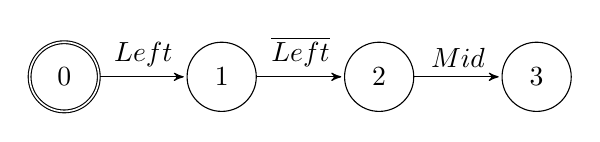
\begin{tikzpicture}[>=stealth',shorten >=1pt,auto,node distance=2cm]
  \node[accepting,state] (S)      {$0$};
  \node[state]         (q1) [right of=S]  {$1$};
  \node[state]         (q2) [right of=q1] {$2$};
  \node[state]         (q3) [right of=q2] {$3$};

  \path[->] (S)  edge   node {$Left$} (q1);
  \path[->] (q1) edge   node {$\overline{Left}$} (q2);
  \path[->] (q2) edge   node {$Mid$} (q3);
\end{tikzpicture}
\end{center}
\newpage
For a Right Turn the signal sequence for the robot to stop rotating is the following:

\begin{center}
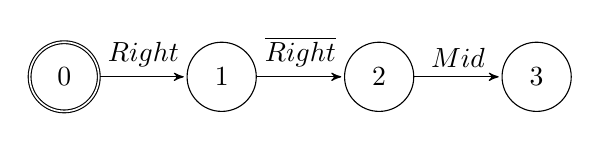
\begin{tikzpicture}[>=stealth',shorten >=1pt,auto,node distance=2cm]
  \node[accepting,state] (S)      {$0$};
  \node[state]         (q1) [right of=S]  {$1$};
  \node[state]         (q2) [right of=q1] {$2$};
  \node[state]         (q3) [right of=q2] {$3$};

  \path[->] (S)  edge   node {$Right$} (q1);
  \path[->] (q1) edge   node {$\overline{Right}$} (q2);
  \path[->] (q2) edge   node {$Mid$} (q3);
\end{tikzpicture}
\end{center}

\FloatBarrier

\section{Path Optimizer}
Once the robot found how the escape from the labyrinth we implement a function able to optimize
the memorized path. This algorithm optimizes how to escape on a shortest and fastest way.\\
In order to solve this task, we implement a truth table with the 9 possible cases to optimize the code. The truth table is described in the following table:\\


\begin{table}[h]
\begin{center}
\caption{Path Corrector Table}
\begin{tabular}{|l|c|}
\hline
\textbf{Possibility} & \textbf{Optimization}\\ \hline
LUL & S\\ \hline
RUR & S\\ \hline
SUR & L\\ \hline
RUS & L\\ \hline
LUS & R\\ \hline
SUL & R\\ \hline
LUR & U\\ \hline
RUL & U\\ \hline
SUS & U\\ 
\hline
\end{tabular}
\end{center}
\end{table}
\FloatBarrier

\begin{figure}[h!!!]
\includegraphics[width=\textwidth]{chart1}
\caption{Flowchart of Path Optimizer}
\end{figure}

The Following  example describes the steps of the process in order to optimize the path file from the maze run described in figure  \ref{fig:maze_example}. We can see how it needs 6 steps, 6 while loops for optimize the path from a sting of 14 characters to just 2 characters.\\\\

Example:
\begin{tabbing}
\= path = [\underline{LUL}LLUSULLUSLL] \quad \= LUL = S \\
\> path = [SL\underline{LUS}ULLUSLL] \> LUS = R\\
\> path = [SL\underline{RUL}LUSLL] \> RUL = U\\
\> path = [S\underline{LUL}USLL]  \> LUL = S\\
\> path = [S\underline{SUS}LL]  \> SUS = U\\
\> path = [\underline{SUL}L]\> SUL = R\\
\> path = [RL] \>
\end{tabbing}

\section{Calibration}
In order to have a proper reading of the path we had to find a threshold value between the path reflectance value and the background reflectance value for each sensor. The threshold value could easily be found by measuring the value in both cases and setting it as the mean value. However, the light environment in which we set the threshold might not be the same as the one we will test the robot on. If the light during the test is very intense, the path might become too bright and the robot might identify it as background. To solve this problem we tested the sensor in various light environments and distances to the floor and found a threshhold that worked in all conditions. We set this value internally in our code. 
\begin{figure}[h]
\includegraphics[width=\textwidth]{calib3}
\caption{The Problem with different light intensities}
\end{figure}



\chapter{Interface}
In our project we use two libraries for the LCD display from Adafruit. Firstly we take a look at the drawMenu function. This function is responsible for drawing the Menu on the LCD display. This function is called every few milliseconds, so if there is a change on the menu this function is responsible for updating the menu on the screen. There is also one very important global variables, the variable menuitem.The menu item remembers the selected menu item. So, if its value is 1, the first menu item is selected, so the drawMenu function must draw this menu item as black with white letters. If the menu item is 2 the second menu item is selected and so on. The menu is composed of 4 desired functions applicable by user: Follow the line, Back to the start, Find the fastest way, Reset. When the user wants to choose one of these functions, he press the button Select.

At first we initialize the global variable and then the display. In the loop function, at first we call the drawMenu function to draw the menu on the screen. Then we read the value from the Button and check if the button is pressed. For example, if we are on the main screen and the first menu item is selected, if the value has increased, the menuitem variable increases and in the next loop the drawMenu function will draw the second menu item as selected. If we now press the button we navigate to the second page, where we set the value of the variable. Again using the button we can increase or decrease the value of the variable.

\chapter{Conclusion}

Taking into account the objectives we stated in the begging of the report (in subsection\ref{subsec:obj}) we were able to sucsed in creating a robot that fullfills that urpose

%%%%%%%%%%%%%%%%%%%%%%%%%%%%%%%%%%%%%%%%%%%%%%%%%%%%%
% Refer�ncias bibliogr�ficas - Registo directo
\addcontentsline{toc}{chapter}{Bibliography} % prep. �ndice
\begin{thebibliography}{99}

\bibitem{latexcompanion} 
ATmega48A/PA/88A/PA/168A/PA/328/P Datasheet

\bibitem{Arduino} 
Arduino - Home
\\\texttt{https://www.arduino.cc/}

\bibitem{citation} 
How to Make a Line Follower Robot in 10 Minutes | DIY Hacking
\\\texttt{https://diyhacking.com/make-line-follower-robot/}

\bibitem{citation} 
AVR LIBC HOME PAGE,
\\\texttt{http://www.nongnu.org/avr-libc/}



\end{thebibliography}


\end{document}
